% MSc thesis style for TU Delft Embedded Networked Systems Group.

% MIT License
%
% Copyright (c) 2019 TU Delft Embedded and Networked Systems Group and Casper Dennis van Wezel.
%
% Permission is hereby granted, free of charge, to any person obtaining a copy
% of this software and associated documentation files (the "Software"), to deal
% in the Software without restriction, including without limitation the rights
% to use, copy, modify, merge, publish, distribute, sublicense, and/or sell
% copies of the Software, and to permit persons to whom the Software is
% furnished to do so, subject to the following conditions:
%
% The above copyright notice and this permission notice shall be included in all
% copies or substantial portions of the Software.
%
% THE SOFTWARE IS PROVIDED "AS IS", WITHOUT WARRANTY OF ANY KIND, EXPRESS OR
% IMPLIED, INCLUDING BUT NOT LIMITED TO THE WARRANTIES OF MERCHANTABILITY,
% FITNESS FOR A PARTICULAR PURPOSE AND NONINFRINGEMENT. IN NO EVENT SHALL THE
% AUTHORS OR COPYRIGHT HOLDERS BE LIABLE FOR ANY CLAIM, DAMAGES OR OTHER
% LIABILITY, WHETHER IN AN ACTION OF CONTRACT, TORT OR OTHERWISE, ARISING FROM,
% OUT OF OR IN CONNECTION WITH THE SOFTWARE OR THE USE OR OTHER DEALINGS IN THE
% SOFTWARE.

\documentclass[10pt,twoside,a4paper,openright]{report}

% add new packages here
\usepackage{algorithm}
\usepackage{algpseudocode}

\usepackage{xcolor}
\usepackage{listings}
\definecolor{backcolour}{rgb}{0.95,0.95,0.95}
\lstdefinestyle{mystyle}{
    backgroundcolor=\color{backcolour},   
    basicstyle=\ttfamily\footnotesize,
    breakatwhitespace=false,         
    breaklines=true,                 
    captionpos=b,                    
    keepspaces=true,                 
    numbers=left,                    
    numbersep=5pt,                  
    showspaces=false,                
    showstringspaces=false,
    showtabs=false,                  
    tabsize=2
}
\lstset{style=mystyle}

\usepackage{subcaption}

\usepackage{todonotes}

% math packages
\usepackage{amsmath}
\usepackage{amssymb}

% textblocks for title page
\usepackage[absolute]{textpos}

% use babel for proper hyphenation
\usepackage[british]{babel}

% Graphics: different for pdflatex or dvi output, choose one
%%\usepackage[dvips]{graphicx}
%%\usepackage[pdftex]{graphicx}
\usepackage{graphicx}

\usepackage{epstopdf}
\usepackage{rotating}
% \usepackage{subfigure}

% Make captions distinguishable
\usepackage[textfont=bf]{caption}

% Chose font style
\usepackage[scaled=.92]{helvet}

% for url's use "\url{http://www.google.com/}"
\usepackage{url}
\usepackage[plainpages=false]{hyperref} 

% Information that will be filled in at various points in the report
\newcommand{\reportTitle}{Dynamic Vital Sign estimation for multiple people using mmWave technology}
\newcommand{\reportAuthor}{Dirk den Hoedt} % Please put your full and official name here: no abbreviations (and to Dutch students: geen roepnamen)
\newcommand{\studentNumber}{4624300}
\newcommand{\reportEmailTUD}{d.denhoedt@student.tudelft.nl}
\newcommand{\reportEmailNonTUD}{dirkdenhoedt@live.nl}
\newcommand{\reportUrlEmailTUD}{\href{mailto:\reportEmailTUD}{\reportEmailTUD}}
\newcommand{\reportUrlEmailNonTUD}{\href{mailto:\reportEmailNonTUD}{\reportEmailNonTUD}}
\newcommand{\reportMSC}{Embedded Systems} % Examples are {Embedded Systems} {Computer Engineering} {Computer Science} or {Electrical Engineering}
\newcommand{\reportDate}{01-09-2022 (TBD)}
\newcommand{\presentationDate}{16-09-2022 (TBD)}
\newcommand{\graduationCommittee}{
Marco Zuniga (chairman) & Delft University of Technology \\
Francesco Fioranelli & Delft University of Technology \\
Caitlin Ramsey MSc & Delft University of Technology \\
Tom Goos & Erasmus MC \\
}

% Provide full name and surname (no abbreviations), so "Koen Langendoen" not "K. Langendoen"

% The order of listing above: 

% title + Graduation committee chairman name and surname (chairman)
% title + Supervisor 1 name and surname (direct supervisor)
% title + Supervisor 2 name and surname (direct supervisor)
% ...
% title + Supervisor X name and surname (direct supervisor) 
% ...
% Others (ordered by title and alphabetical)

% Example: 
% prof.\,dr.\,Koen Langendoen (chairman) & Delft University of Technology \\ 
% dr.\,Przemys{\l}aw Pawe{\l}czak & Delft University of Technology \\ 

\newcommand{\reportAbstract}{WRITE YOUR ABSTRACT HERE}

\newcommand{\reportKeywords}{LIST YOUR KEYWORDS HERE}

% Did the thesis lead to a paper? 
% e.g. The work presented in this thesis has lead to a paper which has been submitted to a conference for publication, pending peer-review
%\newcommand{\reportPaper}{LINE ABOUT YOUR PUBLICATION GOES HERE}
\newcommand{\reportPaper}{}


% Information for pdflatex
\pdfinfo{
/Author (\reportAuthor)
/Title (\reportTitle)
/Keywords (\reportKeywords)
}

\begin{document}

\pagenumbering{alph}
\pagestyle{empty}

% Make frontcover
\include{template/frontcover}

% Set marginns
\hoffset=1.63cm
\oddsidemargin=0in
\evensidemargin=0in
\textwidth=5in

%
\parindent=1em

% Empty page
\cleardoublepage

\pagestyle{plain}
\pagenumbering{roman}
\setcounter{page}{1}

% Create title page: page i (hidden)
\include{template/titlepage}

% Create Graduation Data and Abstract: pages ii and iii (hidden)
\include{template/graduationdata}

% Empty page: page iv
\cleardoublepage

% (Optional) Include quotation: page v (uncomment if needed)
\thispagestyle{empty}

\null\vfill

\begin{center}
\emph{``Never give up, for that is just the place and time that the tide will turn.``} -- Harriet Beecher Stowe
\end{center}

\vspace{10cm}

\clearpage


% Empty page: page vi
\cleardoublepage

% Create preface: page v
\chapter*{Preface}
\addcontentsline{toc}{chapter}{Preface}

% Put a motivation for a research topic here.
Because of my part-time job in the Erasmus MC, I have seen a lot of medical devices, most of them have one or more embedded systems inside of them. Because of my interest both for the embedded systems- and the medical world, I wanted to find a graduation project where both fields came into play. In the Erasmus MC I found Caitlin Ramsey, which did her PhD in the field of contact-less vital signs monitoring of neonates using mmWave radar technology. Caitlin was looking for someone to research the ability to do the vital signs calculations on the chip hardware itself, where currently it was done using post-processing techniques. I was immediately interested in this topic, and after I found Marco Zuniga as my thesis supervisor from the TU Delft, I was ready to get started.

\vspace{1\baselineskip}

I want to thank all the persons that have helped me complete my graduation project. First of all, a special thanks to Caitlin for her great support during this project. I could always come to you with any questions I had, and you always answered them in great detail, both technical questions and more general questions. My thesis would not have succeeded without you. Also a big thanks to Marco. You were always able to keep an overview of the project, and helped me approach the project in an academic way. In moments of doubt, you were a great help to steer me in the right direction and to make the project as enjoyable for me as possible. I also want to thank all of the persons which helped me validate the project. Thank you for your time and patience while sitting very quietly in a chair for 5 minutes. I also want to thank all of the people who supported me along the way. Without your kind and encouraging words, I would have probably stranded somewhere halfway. In that regard, a special thanks to Geeske. You have always been there for me, by celebrating successes, and by cheering me up in difficult times. You always gave me the energy to push through and finish with a great result. 

\vspace{1\baselineskip}

\reportAuthor

\vspace{1\baselineskip}

\noindent
Delft, The Netherlands

\noindent
\today

% Empty page: page vi
\cleardoublepage

% Create tabe of contents: page vii
\tableofcontents

\cleardoublepage

\pagenumbering{arabic}
\setcounter{page}{1}

% Create Introduction: page 1
\chapter{Introduction}
\label{chp:introduction}
% This is the motivation for the whole project
% Features:
% - Problem statement
% - Motivation
% - My contribution
% So, first the problem, some basic explanation about the technical terms and the the proposed solution. First the problem, then cliff in which implementation details can be found (not mentioned), then the implication of my solution.
% - vital signs monitoring is important
% - has various downsides, like the connection with the patient, which could come loose
% - explanation of mmwave
% - explanation vs with mmwave
% - for multiple persons
% - final solution
Vital signs monitoring belongs to one of the standard activities nurses perform to patients in a hospital. This has a very good reason, vital signs can give a good estimation of the state of a patient \cite{mok2015vital}. The most common methods to measure a patients vital signs require physical contact with the patient. A sensor has contact with the skin, and a wire runs from the sensor to another device which shows the heart rate. There are some downsides to this method of measuring. The sensor is always attached, so it could become a discomfort to the patient. Also, the mobility is limited because of the connected wires. Another problem could be that the sensor falls off. When this happens the device goes into an alarm state and produces a loud beep, which is annoying for the patient, especially at night. The nurse must also come and connect the sensor back to the patient.

Millimeter wave radar technology is already in use in the automotive industry \cite{mmwave_automotive}. This type of radar can help to detect other cars on the road. The radar module has antennae for sending the radar waves, and antennae for receiving the radar waves. A property that differentiates millimeter wave (mmWave) radar from other types of radar is the frequency of the transmitted signals. A typical mmWave radar can operate in the 30-300 GHz range. In this range, the length of one wave can be measured in millimeters, which explains the name of this radar type. This radar can detect objects on the road, even in difficult (weather) conditions. 

MmWave radar can not only be used in the automotive industry, it could also be potentially used to estimate the vital signs of a person. The radar signals reflect on large bodies of water. 70\% of the human body consists of water. This means that the mmWave radar signals can reflect on humans, a property that can be exploited to implement the vital signs estimation. When a person breaths, its chest moves up and down. The same goes for the beating of the heart. Every time the heart beats, the chest moves a tiny amount. The mmWave sensor can be setup in such a way that it can detect even those small vibrations of the chest. Using signal processing, those vibration signals can be transformed into a heart rate and a respiration rate. 

Using this method solves various downsides compared to the conventional way of measuring someones vital signs. The main advantage is that the sensor is non-invasive, it has no contact with the patient. This is especially beneficial for burn victims or babies that are born very premature. The patient doesn't even notice that he is being monitored. There are no cables connected to the patient which limit the movement, and no sensors which could fall off the body. 

Depending on the antenna, this technology can have a wide field of view, opening up the possibility to measure multiple people using one radar module. For every person in the field of view of the sensor, a vital signs estimation can be performed. The benefit of this is that multiple persons can be monitored without investing in more hardware.

Using a FCMW radar for vital signs estimation also has its downsides. Radar data is very sensitive to noise, so it can only be used in a low noise environment. Because the sensor is contact-less, and the radar beams are invisible, the signal could be blocked by other persons or objects. Another downside that it is difficult to make distinctions between different persons in the radar data. This makes it hard for the sensor to figure out which vital signs belong to which persons.

The aim of this project is to have a mmWave sensor, which is programmed in such a way that it can detect persons, and measure the vital signs of one or more persons in the field of view of the sensor. All of these calculations will be done on the chip, and not on an external computer. Also, the accuracy of this sensor will be assessed.

\section{Problem statement}
\label{sec:problem_statement}
The system must be able to measure the vital signs of multiple persons in reach of the sensor at the same time. There already are some projects which implement this function, but each has its own downsides. For some projects, the sensor is limited to only measuring one person at the same time. Other projects do succeed in measuring the vital signs of multiple persons at the same time, but only using a post-processing technique. This is not an optimal solution, because most of the time, the patients vital signs are needed right away. 

The goal of this thesis is to implement a system which can measure the vital signs of multiple persons at once in real-time. Also, a thorough validation will be performed on the resulting system, to see if this solution can compete with the existing vital signs measuring solutions.

\section{Objectives}
For the implementation of this project, the Texas Instruments IWR6843ISK is used. This is a mmWave sensor which meets all of the technical requirements set for this project. Firmware for this module can be programmed using an IDE (Integrated Development Environment) provided by Texas Instruments.

From the inital problem statement, a set of technical requirements were established, which you can find below:

\begin{enumerate}
    \item The sensor must be able to generate a heatmap from the radar data of the surrounding area.
    \item The sensor must be able to detect one or multiple persons in this heatmap.
    \item The sensor must be able to estimate the vital signs for up to four detected persons at the same time.
    \item The sensor must compute these vital sign estimations in real-time.
    \item The sensor must be able to track the measured person, such that the measuring continues even if the person moves to another location.
    \item The outcome of the sensor must be displayed in a clear way using a GUI on a computer.
    \item The project must be tested against a trusted measurement, to assess the accuracy of the project.
    \item The project must be tested against a range of different persons, to see if the project performs the same on different kinds of persons.
\end{enumerate}

\section{Outline}
In the introduction, which is Chapter~\ref{chp:introduction}, a brief introduction will be given about the project, along with the problem description and the objectives of this thesis.

Chapter~\ref{chp:background} discusses the background information required to have a good understanding about the fundamental concepts this project is build on. Current vital signs measuring techniques will be discussed, but also some fundamental radar theory will be explained. It contains the explanation of the existing building blocks which are used to build this project, but also related work to this project, with the pros and cons of each work listed.

Chapter~\ref{chp:people_detection} focuses on the dynamic people detection algorithm. This algorithm detects persons in view of the sensor, and performs basic tracking to keep the persons in view and make sure that the vital signs estimation algorithms get the best possible data to work with.

Chapter~\ref{chp:measuring_vital_signs} dives into the actual vital signs estimation functionality of this project. The algorithms used are explained and the program flow specific to the vital signs estimation will be visualized.

Chapter~\ref{chp:realtime_implementation} discusses the real-time implementation of the system. The chip used in this project will be examined and a overview of the program flow of the whole project will be discussed and visualized.

Chapter~\ref{chp:validation} is the validation chapter. Now that a prototype has been built using the knowledge of the previous chapters, the prototype has to be validated against a trusted measurement to assess the accuracy of the prototype.

The last chapter, chapter~\ref{chp:conclusions}, is the conclusion. There are also pointers provided for future work.

During this project, a lot of time has been spend on getting Tx beamforming to work. Sadly, while it should have worked well in theory, in practice it did not perform as expected. Appendix~\ref{app:appendix} goes into more detail about the idea behind Tx beamforming, and while the experiment didn't go as planned, a lot can be learned from this approach to the problem.

% \todo{Add the appendix?}

% Background chapter
\chapter{Background \& Related Work}
\label{chp:background}

In this chapter, the background and related work is discussed. In Section~\ref{sec:background}, fundamental concepts are explained which are used in this thesis. In Section~\ref{sec:related_work} the building blocks are laid out, on which this project has been build.

\section{Background}
\label{sec:background}
% More explanation on the concepts behind the techniques used. Explanation on radar, the chips etc.
% To explain:
% - Heart rate detection methods
% - mmWave technology
% - chirps
% - FFTs
\subsection{mmWave technology}
The type of radar used in this project is the \emph{Texas Instruments IWR6843ISK}, see Figure~\ref{fig:iwr6843isk}. This is a FMCW (Frequency Modulated Continuous Wave) radar. It uses short-wavelength elektromagnetic waves with a frequency of typically between 60-81 GHz, which means that it is legal to use in the Netherlands~\cite{freq_plan}. The TI package that is used in this project is an all-in-one solution. It contains the Tx and Rx analog circuitry to generate and capture the RF signals. It also contains analog-to-digital converters (ADCs), microcontrollers (MCUs) and digital signal processors (DSPs) to make signal processing possible all on the chip. It also has some custom hardware accelerators build in to speed up standard radar calculations, such as the generation of an fast fourier transforms (FFTs).

\begin{figure}[t]
\centering
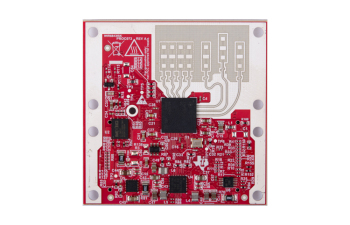
\includegraphics[width=.5\textwidth]{figures/iwr6843isk.jpg}
\caption{The Texas Instruments IWR6843ISK. This module is used throughout the project.}
\label{fig:iwr6843isk}
\end{figure}

\subsubsection{Chirps}
The fundamental concept in radar systems is the transmission of an electromagnetic signal, which is reflected on a target and then received by the radar again. FMCW radars make use of a special kind of signal. The frequency of this signal increases linearly over time, this type of signal is also called a chirp. See Figure~\ref{fig:chirp} for an example chirp waveform, with on the y-axis the magnitude and on the x-axis time. Chirps can be defined by three parameters: frequency ($f_c$), bandwidth ($B$) and duration ($T_c$). A chirp has also a slope ($S$), which captures the rate of change of frequency. There are a lot of parameters which can be set to modify the chirp. In this way the chirp can be tuned to provide information which is important for the application. The main balance which needs to be found is range versus resolution. The signals from the sensor can reach up to 150 meters away, but the resolution will drop to around 4 centimeters. When the sensor is setup to have a range of 2 meters, the resolution can be as low as a couple of millimeters.

\begin{figure}[t]
\centering
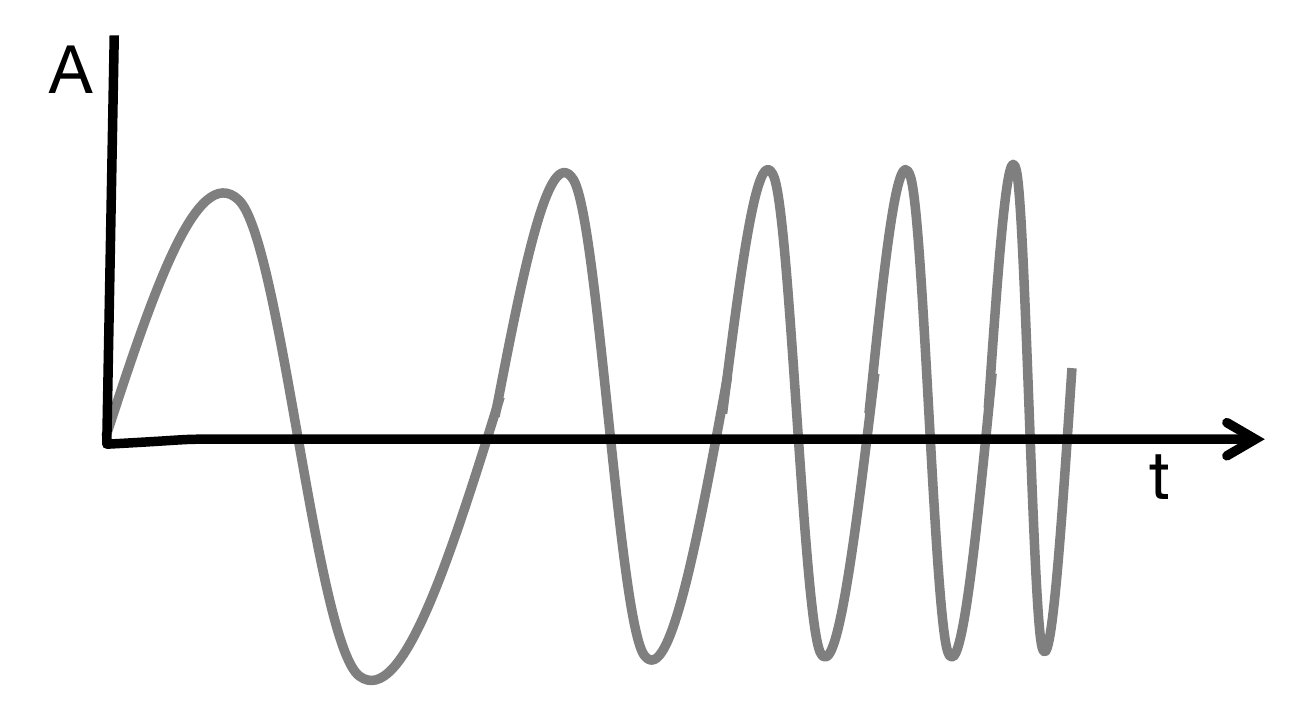
\includegraphics[width=.5\textwidth]{figures/chirp.png}
\caption{Chirp signal, with the amplitude as a function over time.}
\label{fig:chirp}
\end{figure}

\subsection{Range estimation}
In Figure~\ref{fig:fmcw_inner}, a scheme of the inner workings of the FMCW chip can be found. First, a chirp is generated using the synth (1). This chirp is then transmitted over one or multiple Tx antenna (2). When reflected on an object, the signal returns and is captured using the Rx antenna (3). During the travel of the signal, the frequency changes. The further the object is away from the sensor, the more the frequency changes. The signal from the synth and the received signal from the Rx antenna get mixed (4). This mixer has two signals as input, and one signal as an output. The mixer outputs a signal with a frequency which is the difference between the two input frequencies. This output signal is called the intermediate frequency (IF) signal. In Figure~\ref{fig:if_signal} the situation is displayed more visually. Using this information we can use the equation

\begin{equation}
\tau = \frac{2d}{c}
\label{eq:range_equation}
\end{equation}

where $\tau$ is the time delay and $c$ is the speed of light, to compute the distance to the object $d$. 

This is an example where only one object is used. But in the real world, there are almost always more objects to be detected. All of these objects return another reflection, which means that one transmitted signal from the Tx antenna can result in multiple reflections reaching the Rx antenna, as depicted in Figure~\ref{fig:if_multiple}. In this instance, there are multiple IF tones at once, one for each reflected object. To differentiate between those, we make use of a Fourier transform. After processing this Fourier transform, it results in a frequency spectrum in which each peak will point to one separate IF frequency. The IWR6843 has a hardware accelerator to speed up the Fourier transform generation.

% TODO: calculations for distance in meters using FFT?

\begin{figure}[t]
\centering
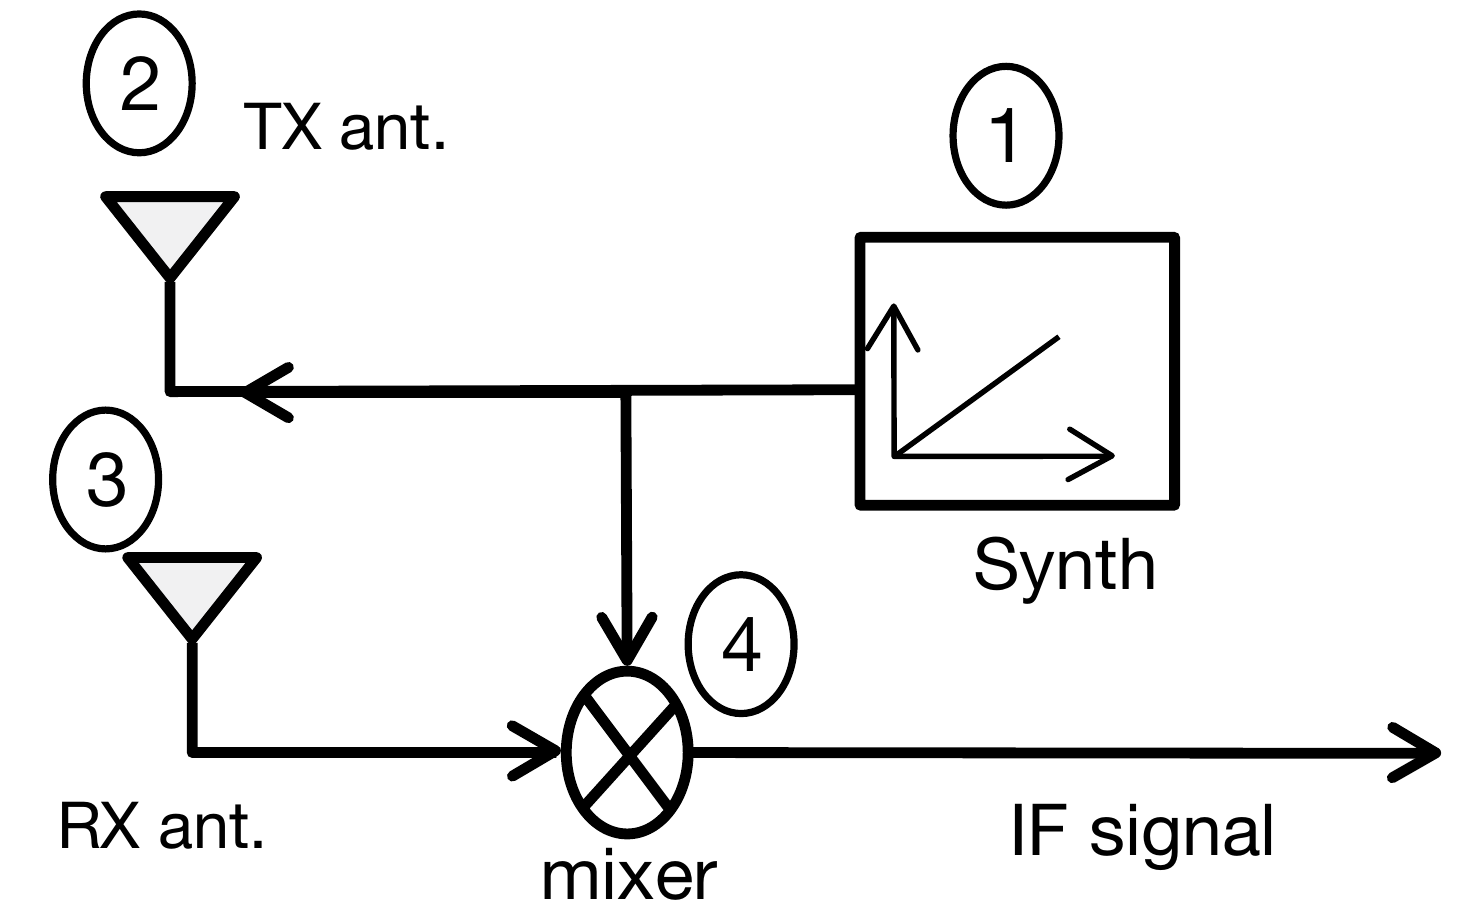
\includegraphics[width=.5\textwidth]{figures/fmcw_internals.png}
\caption{Scheme of the inner workings of the FMCW chip.}
\label{fig:fmcw_inner}
\end{figure}

\begin{figure}[t]
\centering
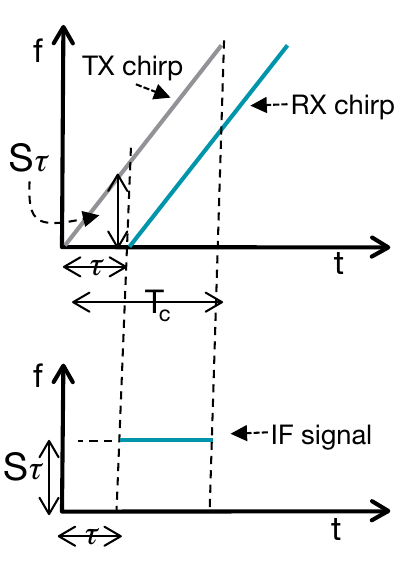
\includegraphics[width=.5\textwidth]{figures/if_signal.png}
\caption{The calculation of the IF signal. In the top graph, the Tx and Rx chirp are plotted. In the bottom graph, the IF signal is plotted.}
\label{fig:if_signal}
\end{figure}

\begin{figure}[t]
\centering
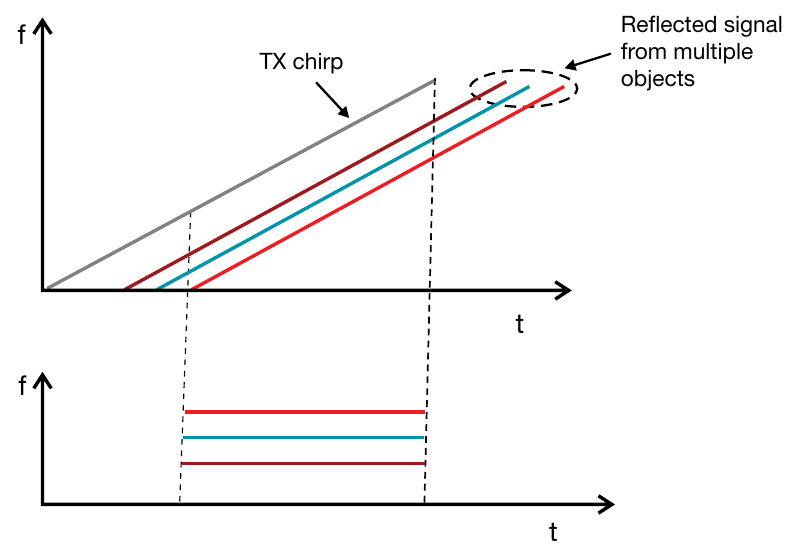
\includegraphics[width=.5\textwidth]{figures/reflected_signals.png}
\caption{One Tx signal can result in multiple reflections on the Rx antennas from multiple objects in front of the sensor.}
\label{fig:if_multiple}
\end{figure}

\subsection{Doppler estimation}
The range information, calculated using the range-FFT, is also known as the 1D-FFT. Most of the time, this is the first processing step for radar data. But, there is more information we can extract from the radar data. Sometimes it is useful to know the velocity of objects. 

To calculate the velocity of objects, we need the data from the range-FFT. The radar transmits two chirps, spaced $T_c$ apart from each other. Both of these chirps get reflected on the object and for both of them a range-FFT is calculated. Because the chirps are transmitted almost immediately after each other, the two FFTs have peaks in the exact same location. What matters now is the phase of the peaks. The output of a FFT is an array of complex numbers. The real part says something about the frequency of the signal, the imaginary part says something about the phase of the sinusoidal signal. The phase between the two chirps is changed slightly because even between those two chirps spaced $T_c$ apart, the object moved. The velocity can be derived using this formula:

\begin{equation}
v = \frac{\lambda \Delta \phi}{4 \pi T_c}
\label{eq:doppler_equation}
\end{equation}

Because the velocity is dependent on the phase value, the velocity could wrap around if the object is moving too fast. Therefore, the maximum speed the radar is able to record before the measurements start to be untrustworthy, is:

\begin{equation}
v_{max} = \frac{\lambda}{4 T_c}
\label{eq:doppler_equation_max_speed}
\end{equation}

To determine the velocities of multiple objects, a FFT is used to differentiate between multiple objects. In the example above for only one object, two chirps are needed to calculate the velocity of the object. To distinguish between multiple objects, more chirps are needed. Each chirp is one input data element for the FFT, so the more chirps, the more accurate the result. All of those chirps together forming the data for the range-FFT and the doppler-FFT are called a frame. 

\subsection{Angle estimation}
Using the methods above, we can estimate the range and the velocity of multiple objects using range- and doppler-FFTs. But, there is still one more shortcoming of these calculations. They only work for one dimension. This means that if object 1 is 3 meters from the sensor and object 2 is 5 meters from the sensor, everything is fine. But, if two objects are at the same distance to the sensor but with a different angle, these two objects would get merged into one. The solution to this problem is to try and calculate the angle of the object with respect to the sensor, also known as the Angle of Arrival (AoA). This way, the data collection from the sensor can be expanded from one dimension into two dimensions.

To calculate the Angle of Arrival, multiple Rx antennas are needed. In Figure~\ref{fig:angle_estimation} the functional diagram of how angle estimation works is displayed. A chirp is emitted from a Tx antenna. The chirp is reflected on an object and received by the first Rx antenna. The distance between the object and the Rx antenna is $d$. When the signal arrives at the second Rx antenna, it has traveled $d + \Delta d$. Because of this $\Delta d$, the phase on the second Rx antenna is different from the first Rx antenna. A similar formula as the doppler estimation can be formed to tie these concepts together:

\begin{equation}
\Delta \phi = \frac{2 \pi \Delta d}{\lambda}
\label{eq:angle_equation}
\end{equation}

Using some basic geometry, we can deduce the formula for the angle of arrival using Eq. \ref{eq:angle_equation}:

\begin{equation}
\theta = \arcsin{\frac{\lambda \Delta \phi}{2 \pi l}}
\label{eq:angle_equation_2}
\end{equation}

Using multiple Rx antennas, in the case of this project using the IWR6843ISK there are 4 antennas, we can calculate the AoA of different objects using a FFT. At this point, a 2D heatmap can be constructed using the calculations from the different estimations above. This heatmap is the starting point for this project.

\begin{figure}[t]
\centering
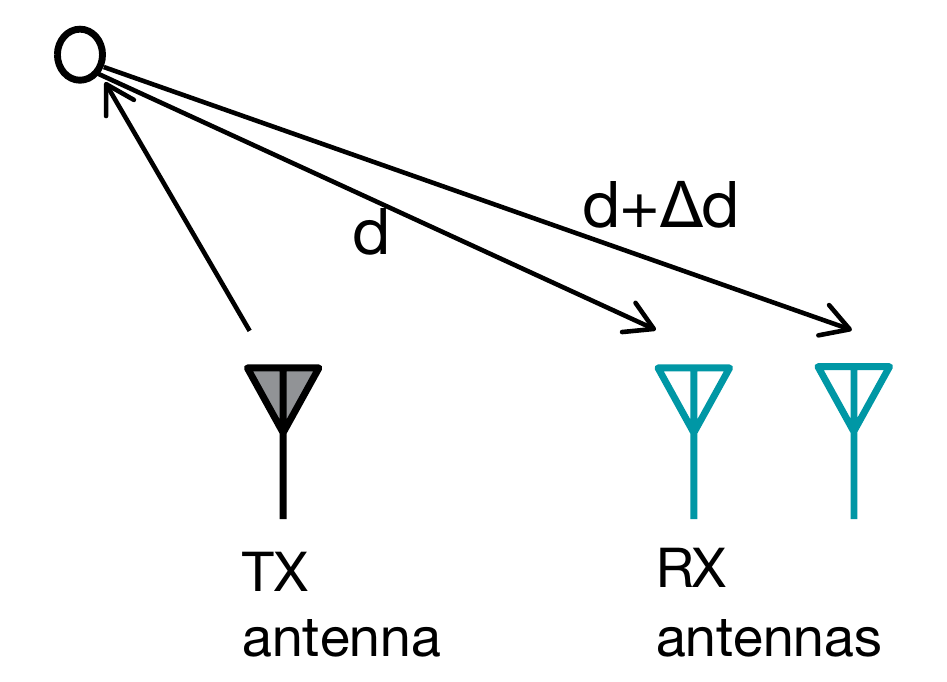
\includegraphics[width=.5\textwidth]{figures/angle_estimation.png}
\caption{One Tx signal is received by multiple Rx antennas. Because the signal travels $\Delta d$ longer to one Rx antenna compared to the other, the angle of arrival can be calculated.}
\label{fig:angle_estimation}
\end{figure}

\section{Related Work}
\label{sec:related_work}
% Use building blocks for the related work. What is new? So start with app1, app2 and app3, and based on these you end up with app4. With app4 you define something novel for example. So, describe this path
% Papers to use:
% - Monitoring Vital Signs Using Millimeter Wave \cite{yang2016monitoring}
% - Vital signs monitoring of multiple people using a FMCW millimeter-wave sensor \cite{ahmad2018vital}
% - Radar remote monitoring of vital signs \cite{li2009radar}
Using radar to estimate vital signs has already been researched before. One of the first papers about the subject is \cite{li2009radar}, which uses a transmitter to send a unmodulated signal to a patient and receive the modulated signal back. The signal gets demodulated and the heart rate and breathing rate can be extracted. In this attempt, a lot of analog hardware is used to make the vital signs extraction work. 

A similar attempt has been made by \cite{yang2016monitoring}. The researchers made use of two separate antennas, one for transmitting and one for receiving. The transmitting antenna does a first sweep through the room by physically moving the antenna to detect persons in the room. After that, the transmitter and receiver can zone in on the person and detect the vital signs of that person. The transmitting and receiving is done with large pieces of equipment. 

In \cite{alizadeh2019remote} the step to FMCW radars can be observed. The authors also use a chip from TI, but an earlier model. They make use of a range-FFT to detect a person, and perform vital signs estimation on that person. A disadvantage of this approach is that the solution is only able to estimate the vital signs of one person. Another disadvantage is that the data gathered by the sensor is send to a computer for processing at a later time. This means that the vital signs estimation is not real time. 

The paper which is closest to the research topic of this paper, is \cite{ahmad2018vital}. The authors from this paper all work for TI, and made a proof of concept solution for multiple person vital signs estimation using a TI sensor. The sensor first looks for persons in the 2D space before the sensor. Then, it uses a special kind of beamforming technique to isolate the data for one person at a time to extract the vital signs. It does this for all of the persons within reach of the sensor. Again, there are some disadvantages with this method. Firstly, the special beamforming technique they are using to isolate the different persons from each other is not shown in detail. When asked if they could share their code, it appeared to be under an NDA. The most important disadvantage is that the calculations are done in Matlab after the data gathering. In the medical world, it is important to have information about a patient right away, and not minutes to hours after they have been recorded. 

% People detection and Rx beamforming chapter
\chapter{People detection}
\label{chp:people_detection}
% Explain:
% - Why this is needed
% - How it is implemented
% - Rx beamforming
% - How it works, maybe some points on the accuracy and how it performs on different types of persons

The first step in dynamic multiple people vital signs estimation, is detecting and tracking persons in range of the sensor. In this chapter, the algorithm to detect persons is explained.

\section{Implementation}
There are existing algorithms to group together multiple points with high energy which are close to each other. These groups of points are an object, a person or any other thing in the space which reflects the RF waves from the sensor. One example is a Constant False Alarm Rate (CFAR) algorithm. This algorithm is already implemented in the mmWave SDK~\cite{mmwavesdk_website}. This is a very difficult algorithm to set up however, it requires intricate knowledge about the inner workings of the algorithm and of all of the right data streams in the chip. Documentation on how to implement this algorithm was missing, only a working general version is provided. Because of these reasons, a detection algorithm was build from scratch. Because it was build from the ground up, it was ensured that all of the needs and output formats could be met.

\subsection{Input data format}
The algorithm returns a list of coordinates with a maximum of 4 persons. It makes use of the build-in range-FFT, doppler-FFT and angle-FFT implementations, described in Section~\ref{sec:background}. Using these methods, a 2 dimentional heatmap can be generated. On the x-axis are all of the bins in the azimuth direction and on the y-axis are all of the bins in the range direction. Each bin contains information about the energy level in that bin. In other words, how much signal reflection has been observed in that bin location. 

% TODO add in schematic view of heatmap generation

\subsection{Noise removal}
Before persons can be detected, the amount of background noise needs to be removed. Because with less noise, the persons in front of the sensor will stand out more and will be easier to detect. Also, the signal strength will be improved. For the vital signs application the sensor is used for in this project, it can be assumed that the sensor will be in a static position, so there will be no background change. For each new background, a new calibration round needs to be done. During this calibration, the sensor will scan the space in front of it. It is very important that no other persons or objects other than static ones are at that moment in view of the sensor. The sensor will scan 64 and take the average of those scans. This noise map will both be saved on the device and returned to the computer via UART. In this way, the computer can send the values along with all of the other parameters when the sensor is restarted, and the calibration round doesn't need to be run again. When the calibration data is in place, it can be used to remove the noise from each new frame that is coming in. This noise algorithm also corrects for whole rows being over saturated. Those rows can be seen clearly in Figure~\ref{fig:no_noise_removal}. The difference between noise correction and no noise correction can be observed in Figure~\ref{fig:noise_vs_no_noise}.

\begin{figure}[t]
\begin{subfigure}{.45\textwidth}
  \centering
  % include first image
  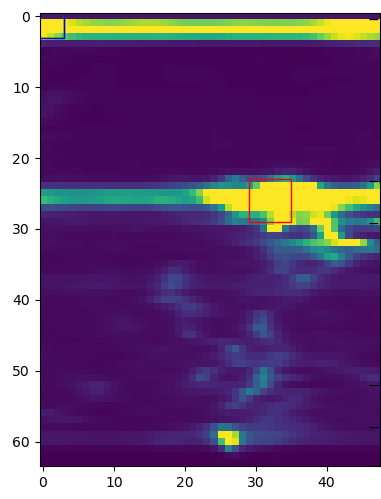
\includegraphics[width=.9\linewidth]{figures/people_detection/heatmap_no_filtering2_crop.png}  
  \caption{Heatmap without any noise removal.}
  \label{fig:no_noise_removal}
\end{subfigure}
\begin{subfigure}{.45\textwidth}
  \centering
  % include second image
  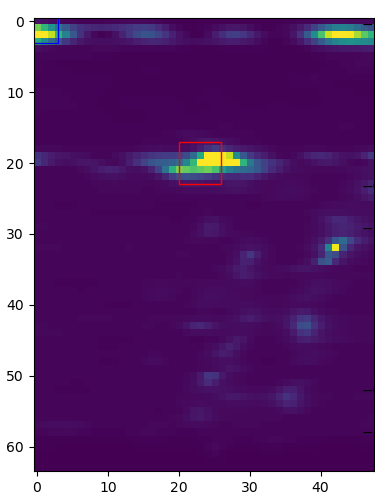
\includegraphics[width=.9\linewidth]{figures/people_detection/heatmap_with_filtering_crop.png}  
  \caption{Heatmap with noise removal implemented.}
  \label{fig:noise_removal}
\end{subfigure}
\caption{These two heatmaps show the difference between noise removal and no noise removal.}
\label{fig:noise_vs_no_noise}
\end{figure}

\subsection{Peak detection}
This algorithm works by detecting peaks. During the testing phase, it was determined what the minimal peak height is for a person in the frame. The maximum heat in one heatmap bin is \emph{32000}. The minimal peak generated by a person in a frame is \emph{2000}. This is the first filter, only the peaks which are higher than the threshold are considered.

For this application, it is assumed that each person is sitting approximately half a meter to one meter apart. This translates in the grouping functionality of the person detection algorithm. For each new peak that is found, it is checked if there has been another peak found within half a meter of the new peak. If that's the case, the peak with the biggest heat will be added to the list. This results in finding the biggest peak for each person, provided they sit half a meter apart. The biggest peak gives the information with the highest SNR value, such that the following algorithms will work in the most optimal form. This algorithm is executed once every 64 frames. Since the program processes around 10 frames per second, every 6.4 seconds there will be another person detection. The algorithm is not run every frame because it takes relatively long to compute, and the whole system is more stable in this way. In the future, it would be best to implement a sliding window and take the average of multiple frames to base the tracking on. For this project that could not be implemented, because there was not enough space on the chip and there was no time left for additional calculations. This could be solved by software optimizations.

\begin{algorithm}
\caption{Person finding algorithm}\label{alg:person_finding_algorithm}
\begin{algorithmic}
\Require $heatmap$
\State $maxPeaks \gets list()$
\For{$x=0,1,\ldots,azimuthLength$}
    \For{$y=0,1,\ldots,rangeLength$}
        \State $bin \gets heatmap(x, y)$
        \If{$bin > 2000$}
            \If{$bin$ heat is larger than surrounding bins}
                \If{bin $c$ in $heatmap$ with distance $<$ 0.5 meter}
                    \If{$bin > c$}
                        \State Add $bin$ to $maxPeaks$
                        \State Remove $c$ from $maxPeaks$
                    \EndIf
                \Else
                    \State Add $bin$ to $maxPeaks$
                \EndIf
            \EndIf
        \EndIf
    \EndFor
\EndFor
\end{algorithmic}
\end{algorithm}

\subsection{Result}
In Algorithm~\ref{alg:person_finding_algorithm}, an overview of the algorithm in pseudo code can be found. The algorithm in itself is not very complicated, but it gets the job done for this use case. Figure~\ref{fig:person_detection_two} shows the heatmap result if two persons are sitting in front of the sensor. The red and yellow boxes are drawn with exactly in the middle the peak that is detected. These peaks will be used internally for vital signs estimation, this is purely a visualization for the user. In Figure~\ref{fig:person_detection_four}, four persons are detected at the same time. This is possible, but it becomes really crowded in this relatively confined space. The most optimal way for the users will be measuring one or two persons at the same time, which will also become apparent later in this thesis. 

% TODO insert conclusion?

\begin{figure}[t]
\centering
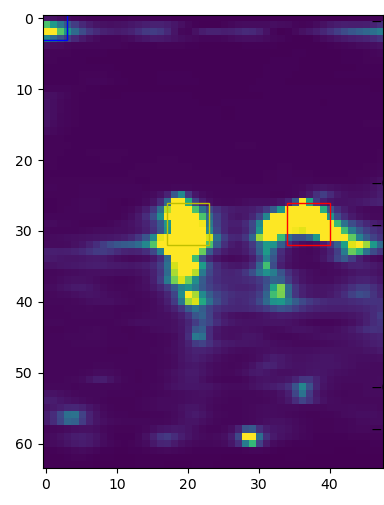
\includegraphics[width=.5\textwidth]{figures/people_detection/multiple_3_crop.png}
\caption{Two persons at the same time detected. Each detected person gets a box drawn around it with a color.}
\label{fig:person_detection_two}
\end{figure}

\begin{figure}[t]
\centering
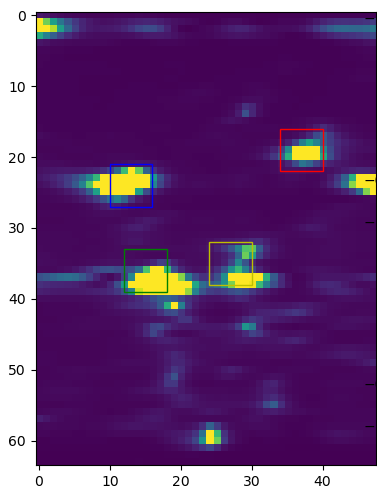
\includegraphics[width=.5\textwidth]{figures/people_detection/4_2_crop.png}
\caption{Four persons at the same time detected. Each detected person gets a box drawn around it with a color.}
\label{fig:person_detection_four}
\end{figure}

% Vital sign extraction and estimation chapter
\chapter{Extracting Vital Signs}
\label{chp:measuring_vital_signs}
% Explain:
% - The phase signal
% - The unwrapping of the phase signal
% - The two different bandpass filters
% - The peak counting
In this chapter, all of the signal processing techniques are explained to get from a selected bin in a heatmap to a heart rate and a respiration rate.

\section{Phase signal}
% - explain the parameters send to the chip
% - explain the accuracy from these parameters
% - explain that is not enough to measure vital signs
% - explain the phase of the signal 
% - explain phase extraction
For accurate vital signs extraction and waveform analysis, the phase of the radar signal is needed. This section explains why the phase signal is needed and how it can be extracted.

\subsection{Radar parameters}
\label{sec:radar_parameters}
Like mentioned in Section~\ref{sec:mmwave_tech}, every time the IWR6843 is restarted, a lot of parameters get send from the computer to the chip to properly setup different parts of the chip. An important part of these parameters are the chirp designs. These parameters among others determine the length of the chirp, the frequency range of the chirp and how many chirps are in one frame. The part of the parameters file which sets up the chirps and the frames can be found in Listing~\ref{lst:parameters}. To better understand how we can extract the vital signs from the radar data, we need to know what the resolution of the data is.

The exact meaning of these parameters can be found in the mmWave SDK documentation~\cite{mmwavesdk_website}. The ones important for this section are summarized in Table~\ref{tab:parameters}.

\begin{table}[t]
\centering
\begin{tabular}{|l|c|}
\hline
Parameter & Value \\ \hline
Ramp End Time (us) & 40 \\
Frequency slope (MHz/us) & 98 \\
Start Frequency (GHz) & 60 \\
Number of ADC samples & 64 \\ \hline
\end{tabular}
\caption{Some of the parameters from Listing~\ref{lst:parameters} with their value.}
\label{tab:parameters}
\end{table}

To determine the range resolution for the parameters used in this project, we make use of the formula provided by TI \cite{range_est_training_website}, as seen in Eq.~\ref{eq:range_res_equation}.

\begin{equation}
d_{res} = \frac{c}{2 B}
\label{eq:range_res_equation}
\end{equation}

Where $B$ is the bandwidth of the chirp in Hz, and $c$ is the speed of light in m/s. $B$ can be calculated by multiplying the slope of the chirp and the duration of the chirp, see Eq.~\ref{eq:b_calc}.

\begin{equation}
B = S \times T_c = 98 \times 40 = 3920 MHz
\label{eq:b_calc}
\end{equation}

Using Eq.~\ref{eq:range_res_equation}, it can be calculated that the resolution from the sensor is approximately 3.8 centimeters. The maximum range can also be calculated, by using Eq.~\ref{eq:range_max_equation}.

\begin{equation}
d_{max} = \frac{c A}{2 B}
\label{eq:range_max_equation}
\end{equation}

Where $A$ is the number of ADC samples which are taken for each chirp. Using this formula, the maximum range that the sensor can reach using these parameters is 2.45 meters. 

Bin resolution is too large for vital signs estimation. If a person is breathing, the chest only moves one millimeter or less, while the bin resolution is multiple millimeters. The heartbeats are even more fine grained, the movement of the chest for one heartbeat could even be fractions of millimeters. Therefore, another technique must be used to reach the resolution needed for vital signs estimation. When the radar data is processed into a FFT, the output is an array of complex numbers. This complex number not only says something about the magnitude of the input data, but also something about the phase of the input data. See also Figure~\ref{fig:phase_difference}. This phase is how the reflected waveform returns to the sensor. When nothing happens to the chest, this phase stays the same. But if the heart is in the middle of a beat, the chest is tens of millimeters closer to the sensor. These tens of millimeters result in a phase shift. This is data that can be used to estimate vital signs. 

\begin{figure}[t]
\centering
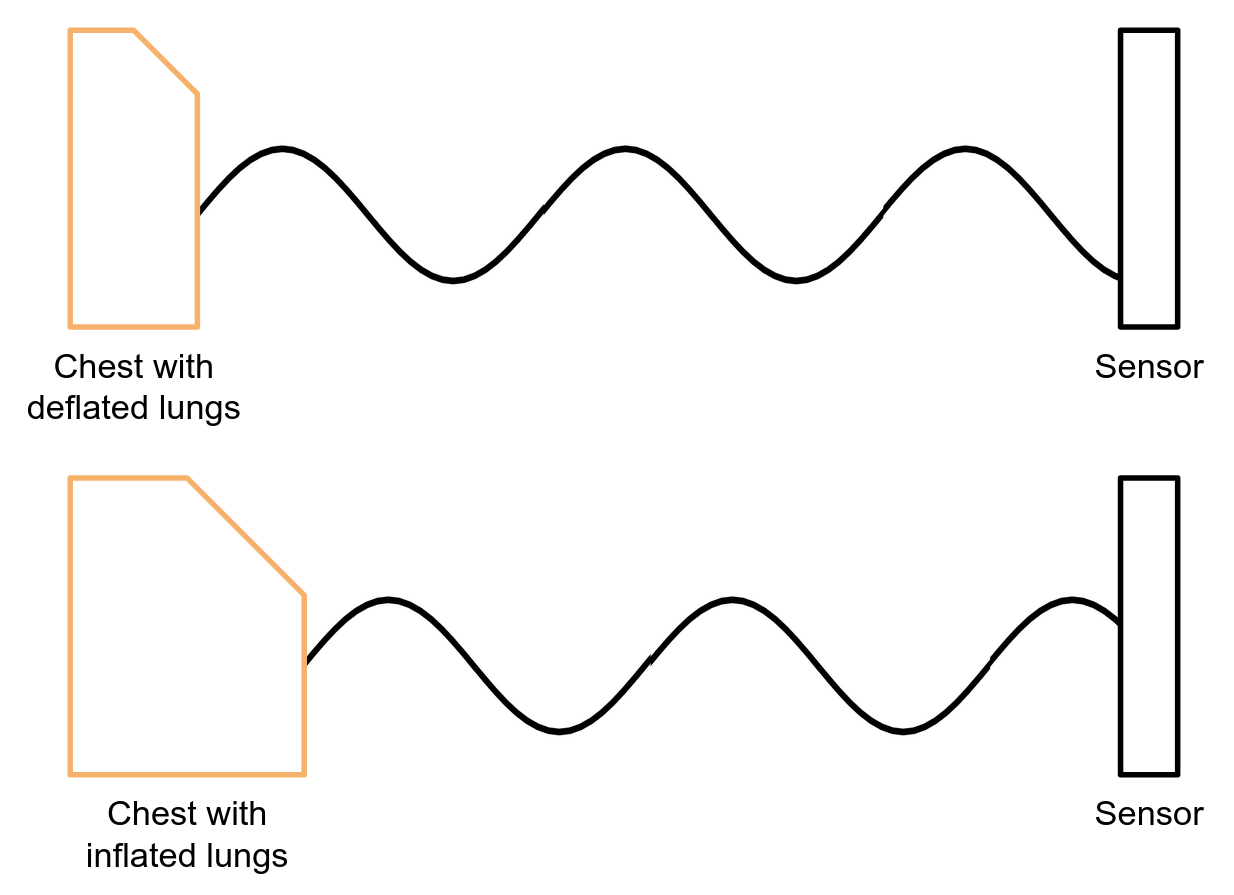
\includegraphics[width=.7\textwidth]{figures/measuring_vital_signs/phase_difference.png}
\caption{Exaggerated scheme on how the phase of the signal changes depending on the inflated or deflated chest of a person.}
\label{fig:phase_difference}
\end{figure}

\subsection{Phase unwrapping}
% - formula with the tan
% - unwrapping because of 2 pi
% - calculating the doppler?
Most existing solutions, like~\cite{li2009radar, yang2016monitoring, alizadeh2019remote} make use of phase extraction like in Figure~\ref{fig:phase_unwrapping}. From the radar data the range-FFT is calculated, on this FFT the peak is found. This peak denotes the location of the person, see also Figure~\ref{fig:ti_fft}. From that peak the phase is extracted and saved in a sliding window configuration. This same event repeats every 50 milliseconds. So, for each 50 milliseconds, the phase is extracted. All of these phase values form a waveform on their own, which can function as the input for the vital signs estimation. 

\begin{figure}[t]
\centering
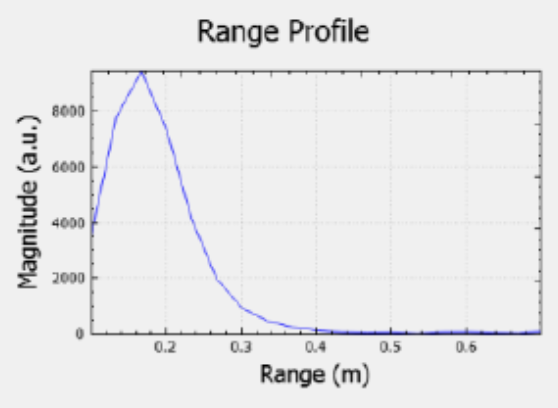
\includegraphics[width=.5\textwidth]{figures/measuring_vital_signs/ti_range_fft.png}
\caption{Person detection using only the range-FFT. This screenshot has been taken from a TI demo.}
\label{fig:ti_fft}
\end{figure}

In the case of this project, the phase must be extracted from the generated heatmap. However, this means that the radar data is put through two more FFTs other than the range-FFT, namely the doppler-FFT and the azimuth-FFT. There were some concerns that the phase information would be lost during the generation of those two other FFTs, but during testing, it became apparent that the vital signs waveform could also be extracted from the phase of one bin in the heatmap. This phase information is retained through the generation of the doppler-FFT and the angle-FFT. Because this is possible, information from a 2 dimensional space can be taken and processed to extract the vital signs. This is the second very important step that needs to be taken to arrive at the multiple person vital signs tracking goal. The first step is to track the persons in the radar view. This second step is to extract and unwrap the separate phase waveforms for each person. The next step is to take these waveforms and extract the vital signs data out of this waveform.

\begin{figure}[t]
\centering
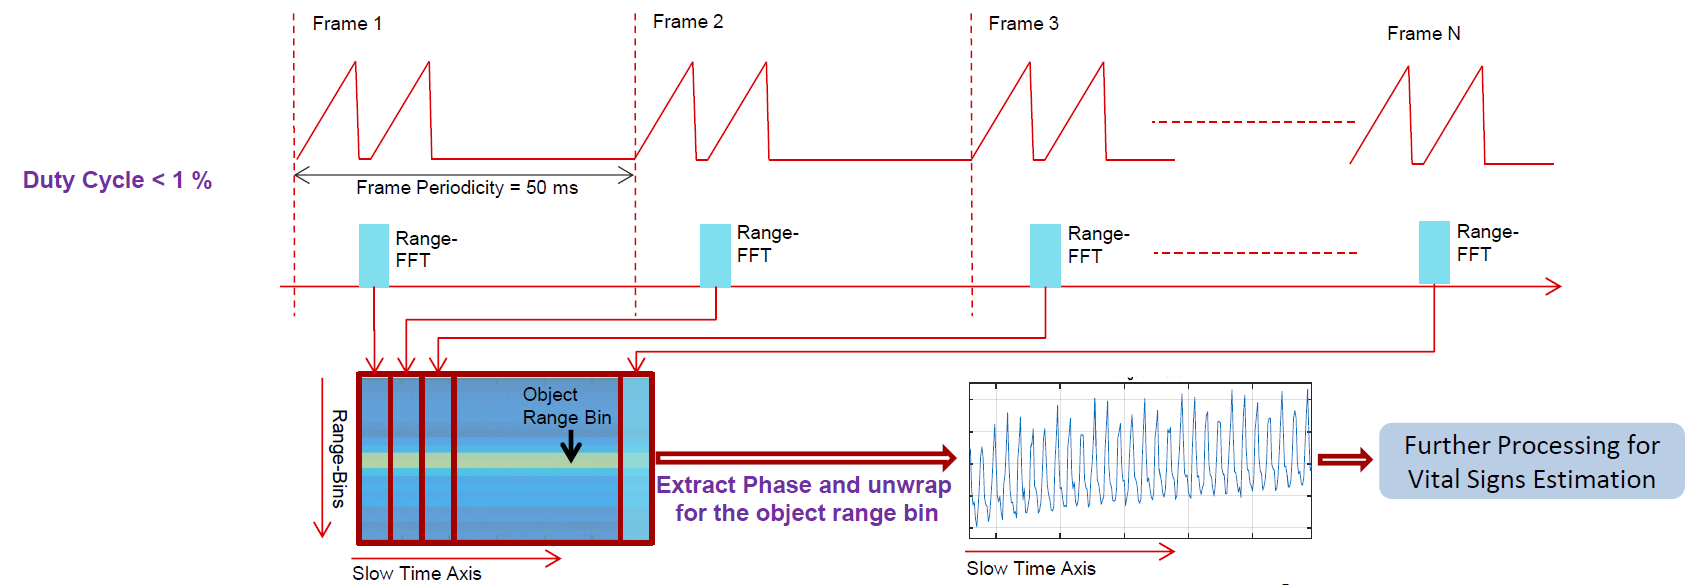
\includegraphics[width=.95\textwidth]{figures/measuring_vital_signs/phase_unwrapping.png}
\caption{Visual representation of how the phase gets unwrapped. Image has been taken from~\cite{vital_signs_lab_website}.}
\label{fig:phase_unwrapping}
\end{figure}

\section{Vital signs estimation}
\label{sec:vit_signs_est}
% - difference is used between different phase values
% - Impulse noise filter
% - IIR biquad filter
% - breath circular buffer
% - heart circular buffer with motion detection
% - peak counting heart with filters
% - peak counting breath with filters
% - execute FFT on the breathing and heart rate estimation
% - peak counting and sorting again
Before starting with this section, I want to emphasize that I have copied these vital sign estimation implementations to a large extend from the TI Vital signs estimation demo~\cite{vital_signs_lab_website} and the Matlab implementation from my mentor Caitlin Ramsey~\cite{caitlin_msc_thesis_2020}. The main alterations I made was to make the code usable for multiple people at the same time. I chose for this approach because I am not very familiar with signal processing given my Embedded Systems background, so it is difficult to innovate in that field. Secondly, the main bulk of code is already implemented for this embedded platform. I think it is important to explain the inner workings of this vital signs estimation implementation in this thesis, because it has a great significance to the project.

% TODO explain the contents of this section

\subsection{Data preparation}
The phase values coming from the heatmap are stored in circular buffers for further processing. But first, the data needs to be prepared. The algorithms work by using the phase changes. A phase change is computed by comparing the current phase by the previous phase value, like in Eq.~\ref{eq:phase_difference}.

\begin{equation}
    \label{eq:phase_difference}
    P_{change} = P_{current} - P_{previous}
\end{equation}

This results in an array with phase changes which can be used in processing. But first, the signal is cleaned up by an impulse noise filter. The data which is coming from the sensor is raw data. There can be unwanted spikes in the data, for example due to electromagnetic interference. This noise needs to be filtered out beforehand. This is done in a sliding window configuration, where the three most recent values are stored. If the ratio between the first and the second, and the ratio between the third and the second are above a certain threshold, the second value will become an interpolation from the first and third value. Figure~\ref{fig:phase_spike_filter} has a more clear visual representation. This filter makes sure that there are no sudden peaks in the data, but that the signal is still able to change shape. Now that the signal is cleaned up, the next step is to differentiate between the heart rate and the respiration rate.

\begin{figure}[t]
\centering
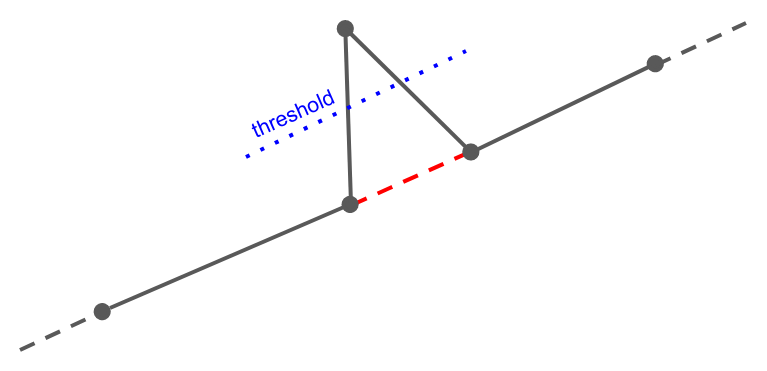
\includegraphics[width=.7\textwidth]{figures/measuring_vital_signs/threshold_interpolation.png}
\caption{Visual representation of how sudden spikes get filtered out of the phase waveform.}
\label{fig:phase_spike_filter}
\end{figure}

\subsection{Splitting the heart rate and respiration rate signal}
To do separate analysis on the respiration rate and the heart rate, the source waveform needs to be separated into two separate waveforms. The way this is done, is by using an IIR filter.

IIR filters are one of two common digital signal processing (DSP) filter types~\cite{iir_info_website}. IIR stands for Infinite Impulse Response. The other common type is the Finite Impulse Response filter. These types of filters modify the frequency content of a signal. FIR filters and IIR filters are both part of the Linear Time Invariant (LTI) filter group. LTI filters can modify the phase and the amplitude of certain frequencies of a signal. These filters are most commonly used to remove undesired frequencies from an input signal. For example: the antenna of a car receives all of the radio stations at once, from 88 MHz to 108 MHz. To make it possible to only listen to a station at for example 89.9 MHz, a filter can be used to only allow the signal with a frequency of 89.9 MHz. The main difference between FIR and IIR filters, is that the IIR filters make use of a feedback mechanism. If the IIR filter is first zero and receives a 1 as an input, the filter output can (theoretically) never reach zero again. A FIR filter works with a certain amount of stages, and is able to reach zero after a certain amount of time. For this project an IIR filter is chosen because it is more efficient to implement for embedded devices, since it uses less memory and calculations compared to a similar FIR algorithm~\cite{iir_faq_website}. 

The IIR filter used in this project is an biquad cascade IIR algorithm. Biquad stands for biquadratic, which refers to the Z-domain, where the transfer function is a ratio of two quadratic functions:

\begin{equation}
\label{eq:biquad_filter_z}
    H(z)={\frac {b_{0}+b_{1}z^{-1}+b_{2}z^{-2}}{1+a_{1}z^{-1}+a_{2}z^{-2}}}
\end{equation}

The filter used in this project can be written down as an equation:

\begin{equation}
\label{eq:biquad_filter}
    y[n]=b_{0}x[n]+b_{1}x[n-1]+b_{2}x[n-2]-a_{1}y[n-1]-a_{2}y[n-2]
\end{equation}

\begin{figure}[t]
\centering
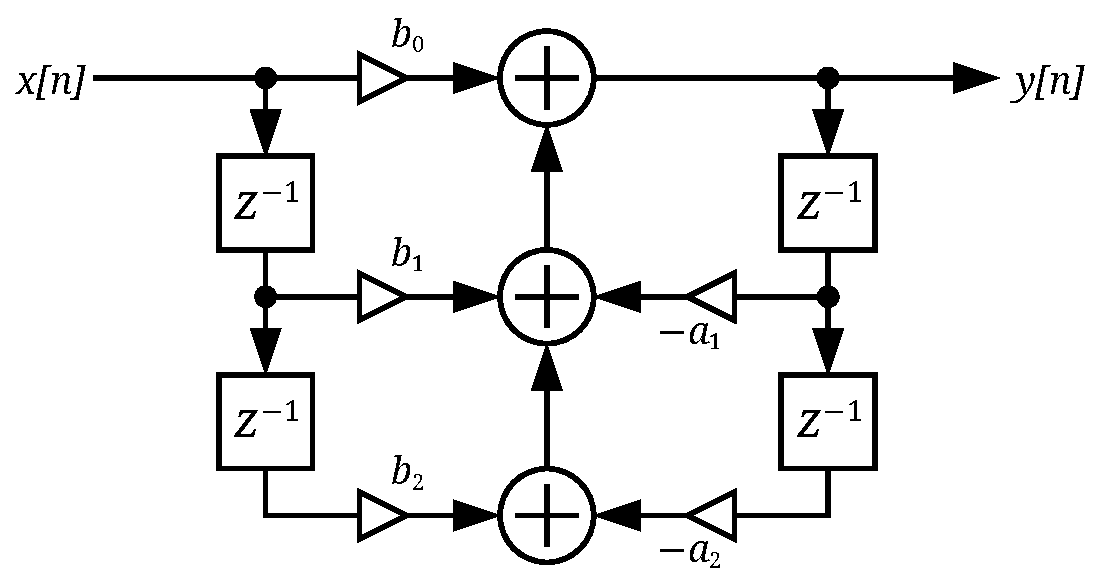
\includegraphics[width=.95\textwidth]{figures/measuring_vital_signs/Biquad_filter_DF-I.pdf}
\caption{The flow graph for a biquad cascade IIR filter. A more visual representation from Eq.~\ref{eq:biquad_filter}, how the input gets transformed to the output.}
\label{fig:iir_visual}
\end{figure}

A more visual flow graph can be found in Figure~\ref{fig:iir_visual}. This algorithm is translated in C code. This filter is executed on the input signal two times, once for the respiration rate waveform and once for the heart rate waveform. The filter is therefore configured like a bandpass filter. It will remove frequencies which are not in the allowed frequency range. The frequency ranges that were used in this project can be found in Table~\ref{tab:freq_ranges}.

\begin{table}[ht]
\centering
\begin{tabular}{|r|c|c|}
\hline
\textbf{Parameter} & \begin{tabular}[c]{@{}l@{}}\textbf{Minimum}\\ \textbf{frequency}\end{tabular} & \begin{tabular}[c]{@{}l@{}}\textbf{Maximum} \\ \textbf{frequency}\end{tabular} \\ \hline
Respiration rate & 0.1 Hz & 0.5 Hz \\
Heart rate & 0.8 Hz & 2.0 Hz \\ \hline
\end{tabular}
\caption{Typical frequency ranges from the respiration rate and heart rate. These frequency ranges are used in this project to filter out the right waveforms to do analysis on.}
\label{tab:freq_ranges}
\end{table}

So, there was one input waveform, which is now split into two different waveforms, one for heart rate and one for respiration rate. The next step is to concentrate on getting a beats per minute (BPM) reading out of this data.

\subsection{Circular buffers}
\label{sec:circular_buffers}
The data from these two separate waveforms are both stored in a circular buffer. This circular buffer acts like a sliding window. Based on the waveform in this buffer, the respiration rate and heart rate can be estimated. The length of these buffers are sent via the configuration file, as can be seen in Table~\ref{tab:vs-parameter-config}. In this table, all of the vital sign parameters are listed, along with their value and a short explanation.

The buffer length is a balancing act. The more data is in the buffer, the more data can be input to the FFT and the more accurate the result will be. But, the longer the buffer is, the more data gets averaged together. This means that instantaneous changes in heart rate frequency will not be visible in the output data. This project makes use of a respiration waveform buffer of 256 data points. A measurement will be taken every 50ms, this is also the frame periodicity, as can be found in Listing~\ref{lst:parameters}. The total buffer length in seconds can also be calculated, as in Eq.~\ref{eq:buffer_length}.

\begin{equation}
\label{eq:buffer_length}
    256 * 50{ms} = 12800{ms} = 12.8 {seconds}
\end{equation}

Which means that a full buffer with respiration data will contain 12.8 seconds of data. Since the heart rate waveform has less amplitude because the chest doesn't move as much and the heart rate is faster than the respiration rate, the buffer is twice as long, resulting in a total buffer length of 25.6 seconds. This is done because we need more accuracy for the heart rate.

Because the heart rate is so fine grained, the heart rate waveform is added in chunks to the buffer. If the chunk is too noisy, for example because the subject is moving a little bit, the chunk gets skipped. This mechanism makes sure that the waveform is as noise free as possible.

\begin{table}[ht]
\centering
\begin{tabular}{|r|c|l|}
\hline
\textbf{Parameters} & \textbf{Values} & \textbf{Comments} \\ \hline
Start range (meters) & 0.3 & \begin{tabular}[c]{@{}l@{}}The persons to be detected \\ are expected to be within \\ the start range and the end \\ range from the sensor.\end{tabular} \\ \cline{1-2}
End range (meters) & 0.9 &  \\ \hline
Respiration waveform size & 256 & \begin{tabular}[c]{@{}l@{}}Specifies the number of points \\ within the waveforms. The \\ more data points are in the \\ circular buffer, the more data \\ is captured and the more \\ accurate the reading becomes. \\ A downside of using a large \\ waveform size is that it looses \\ the ability to capture \\ instantaneous changes.\end{tabular} \\ \cline{1-2}
heart rate waveform size & 512 &  \\ \hline
Rx-antenna to process & 4 & \begin{tabular}[c]{@{}l@{}}Because there are 4 Rx antenna, \\ this value could be max. 4. \\ Because for this implementation \\ the rangeAzimuth-FFT is used, \\ only a value of 4 is allowed.\end{tabular} \\ \hline
\begin{tabular}[c]{@{}r@{}}Alpha filter value for \\ Respiration waveform\\ energy computation\end{tabular} & 0.1 & \begin{tabular}[c]{@{}l@{}}Alpha filter values for recursive \\ averaging of the waveform \\ energies based on the equation \\ below where $x(n)$ is the current \\ waveform value while $E(n)$ is the \\ energy. \\ $E(n)=\alpha x^2(n)+(1-\alpha)E(n-1)$\end{tabular} \\ \cline{1-2}
\begin{tabular}[c]{@{}r@{}}Alpha filter value for \\ heart rate waveform\\ energy computation\end{tabular} & 0.05 &  \\ \hline
\begin{tabular}[c]{@{}r@{}}Scale factor for the \\ Respiration waveform\end{tabular} & 300000 & \begin{tabular}[c]{@{}l@{}}Scaling factors to convert \\ waveform values in floating \\ points to 32-bit integers \\ required for the FFT.\end{tabular} \\ \cline{1-2}
\begin{tabular}[c]{@{}r@{}}Scale factor for the \\ heart rate waveform\end{tabular} & 300000 &  \\ \hline
\end{tabular}
\caption{Overview of all of the Vital Signs configuration parameters getting send to the chip. These parameters mostly control the sensitivity of the chip. For each parameter, the value used in this project is mentioned and a short explanation. }
\label{tab:vs-parameter-config}
\end{table}

\subsection{Peak counting}
\label{sec:peak_counting}
The next step in the algorithm is the peak counting. Both waveforms are filtered, this means that for the respiration waveform there is only a peak when the chest is deflated and then inflated. For the heart rate waveform, there would be a peak for each beat of the heart. This peak counting is only a simple algorithm. For each three consecutive values, it checks if the middle value is bigger than the value on the left or on the right. If it is, a peak has been detected. An additional threshold filter is executed over the peaks to eliminate the invalid peaks.

Since it is known how many peaks there are in the waveform, and it is known how much time a full waveform buffer takes (see Section~\ref{sec:circular_buffers}), the BPM could be calculated. For example, 28 peaks are detected. From Section~\ref{sec:circular_buffers} it is known that a full waveform buffer takes 25.6 seconds. With a simple calculation the estimated heart rate will be revealed, see Eq.~\ref{eq:heartrate_calc}.

\begin{equation}
\label{eq:heartrate_calc}
    \frac{28 * 60}{25.6} \approx 66 {BPM}
\end{equation}

For the respiration rate, Eq.~\ref{eq:heartrate_calc} can be repeated in a similar way. Let's assume 6 peaks are detected in the respiration waveform, see also Figure~\ref{fig:breath_peak_counting}. From Section~\ref{sec:circular_buffers} it is known that the full respiration rate buffer takes 12.8 seconds of data, so:

\begin{equation}
\label{eq:breathrate_calc}
    \frac{3 * 60}{12.8} \approx 13 {BPM (Breaths Per Minute)}
\end{equation}

The algorithm is completed.

\begin{figure}[t]
\centering
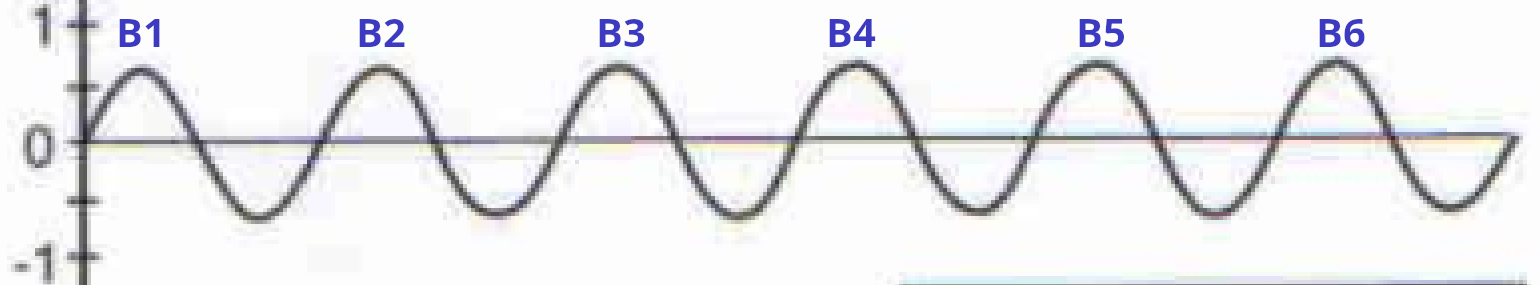
\includegraphics[width=.8\textwidth]{figures/measuring_vital_signs/breath_peak_counting.png}
\caption{This waveform could represent the respiratory waveform in the circular buffer. This waveform spans 12.8 seconds of data. 6 peaks can be detected, each peak is one breath.}
\label{fig:breath_peak_counting}
\end{figure}

\subsection{Executing FFTs on the waveforms}
There is however another option that can be tried. The peak counting method from Section~\ref{sec:peak_counting} is a bit rudimentary. Peaks are detected and filtered, but there could still be false positives or false negatives in this workflow. It would be best to execute a FFT on the waveform and extract the most present frequency from the FFT. Luckily, the chip is specialized in calculating FFTs. Each of the two waveforms is put through the FFT generation, and from each FFT output, the biggest peak is extracted. From this biggest peak, the BPM value can be calculated in a similar way as in Eq.~\ref{eq:heartrate_calc} and Eq.~\ref{eq:breathrate_calc}. Because this method is more advanced and less prone to errors, the outcome of the FFT method can in general be better trusted than the outcome of the peak counting method in Section~\ref{sec:peak_counting}. Both of these methods, peak counting and FFT generation, are applied at the data to end up with the vital signs. For the results of this project, the outcome from the FFT method is used.

% Chapter about the real-time implementation aspect
\chapter{Real-time implementation}
\label{chp:realtime_implementation}
% Explain:
% - Why a real time system is needed
% - The architecture of the chip
% - How we achieve real time performance by using different specialized tools from the chip

In this chapter, the functionality of the chip is explored, an the general program flow is discussed.

\section{Overview}
% This part will be written last
A big part of the innovation of this thesis is implementing all of the calculations on the chip itself. The chip comes equipped with a RF front-end, two processors and other hardware which must all work in unison to do all of the calculations in time, see also Figure~\ref{fig:iwr6843_inner} for the block diagram of the chip. Before the coding can start, the programmer needs to have a good knowledge of how all of the elements in the chip need to work together.

\section{How it works}
% Why is a real time system needed
In a clinical environment, real-time devices have become indispensable. To give a patient the best care possible, vital signs need to be monitored. These vital signs need to be available right away, because if the patients condition is deteriorating, immediate action is from the utmost importance. There are several examples of real-time clinical measurements. Monitoring of the heart with an ECG, heart rate and oxygen levels in the blood using a pulse-oxygen sensor. But also blood pressure, body temperature and respiration rate can be measured in real-time.

Because this real-time aspect is so important, it also is a big design goal for this project. As can be read in Section~\ref{sec:related_work}, there are some implementations which can measure the vital signs of multiple people using only one radar, but all of those methods are using a post-processing technique. This means that the data is first gathered using the radar and captured with a capture card. At a later stage, all of this data is analyzed and the vital signs are extracted. So there are vital signs measured, but they are available far too late from a clinical point of view. The implementation from this project is focusing on the immediate availability of the vital signs which are being recorded at that moment using the radar. In this chapter the designs, elements and techniques are highlighted to process these relatively large amounts of data using a low power chip.

\section{Building blocks}
\label{sec:building_blocks}
The IWR6843 chip consists of two processors. One is a ARM Cortex R4F processor with a clock speed of 200 MHz. The other one is a Digital Signal Processor (DSP) specific C674x processor, made by TI. These two processors are separated into two sub-systems: the main sub-system and the DSP sub-system. See also Figure~\ref{fig:iwr6843_inner}.

\subsection{Main sub-system}
The Cortex R4F processor is the generic all purpose processor in the system. This processor has a managing role in the system. The R4F is connected to all of the communication interfaces, like SPI, I2C, UART and CAN. It is also connected to the radio front-end of the chip. Via a special mailbox system it is also connected to the DSP. 

The main sub-system (MSS) is responsible for all non digital signal processing tasks. It catches the chirp- and frame-interrupts from the radio front-end, and communicates them to the DSP. It also takes care of communicating with external devices. In the case of this project, UART is extensively used to communicate the measurement details with a computer. Another use case for the R4F are more general calculations on the radar data. The DSP takes all of the raw radar data in and processes it to a radar cube. In this radar cube are points in 3 dimensional space, which are detected by the radar. The R4F has also access to this data, and could perform additional algorithms on this data, like object detection, point grouping or even AI techniques.

\subsection{DSP sub-system}
The DSP sub-system (DSS) is responsible for the transformation between the raw ADC radar data and usable data for further processing, for example in a radar cube format. The DSS has also a hardware accelerator build-in, to be able to do specific radar signal processing steps as fast as possible. The Radar Hardware Accelerator (HWA) enables off-loading the burden of certain frequently
used computations in FMCW radar signal processing from the main processor. FMCW radar signal processing involves the use of FFT and log magnitude computations to obtain a radar image across the angle, velocity, and range dimensions. This gives the flexibility of doing common calculations using the HWA, but still design your own algorithms.

The DSP has L1 and L2 caches to store and load calculations quickly. The L3 cache is shared with the MSS, and contains all of the radar data. 

\subsection{Inter-processor communication}
Because the MSS and the DSS are separate processes but must be working in unison, there is a communication technique present in the chip called the \emph{mailbox}. Using this mailbox, messages can be sent from one processor to the other, and vice versa. When a message arrives at a processor, an interrupt is triggered and the message can be processed. Another way to use this method is to use it for processor synchronization. Quite often, the two processors need to be in the same state to proceed to the next part of a calculation. When the two processors are synchronized using the mailbox, they both are at a known state in the program flow and can continue with the task at hand. See as an example Figure~\ref{fig:mailbox_principle}. The processors are starting separately, and are doing each their own initialization routine. After that routine is finished, they are waiting on each other (synchronized). Then they can start the program execution at exactly the same time. An example of sending a message from one processor to another is also given in Figure~\ref{fig:mailbox_principle}.

\begin{figure}[t]
\centering
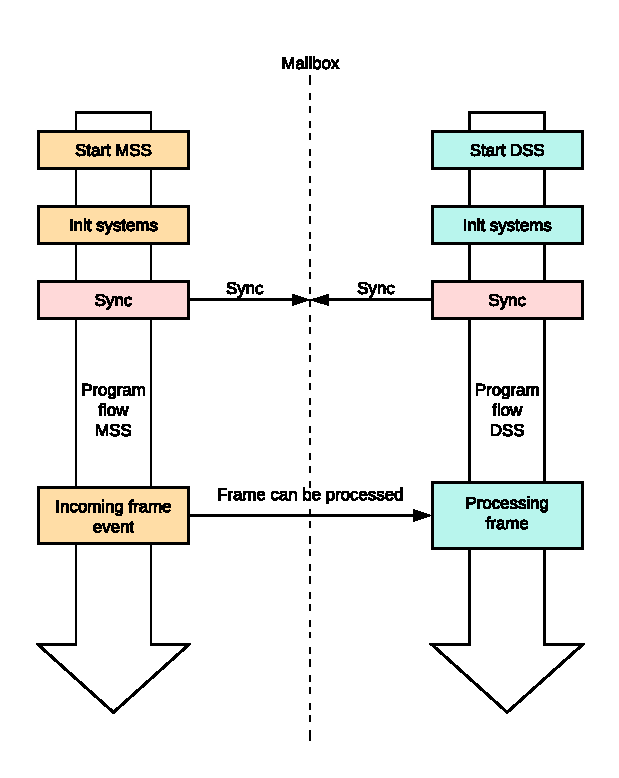
\includegraphics[width=.6\textwidth]{figures/realtime_implementation/Mailbox working principle.pdf}
\caption{Example of the mailbox principle. After startup and initialization, the two processors are synchronized such that they start at the same time. When a frame event ends up at the MSS, it can send a message using the mailbox to the DSS.}
\label{fig:mailbox_principle}
\end{figure}

\section{Implementation}
This section goes into the program flows which make it possible to have real-time vital signs monitoring for multiple persons which are sitting in front of the sensor. A high-level overview can also be found in Figure~\ref{fig:program_flow}.

Like mentioned in Section~\ref{sec:building_blocks}, the IWR6843 contains two processors, one generic ARM processor and one TI DSP. These processors are programmed separately, but the program flow is intertwined, both processors depend on each other to send and receive information. 

\subsection{MSS program flow}
The program starts with an initialization phase, in this phase the processor gets setup to send and receive information from the right locations. The next step is to wait for the CLI input. The IWR6843 receives commands from the connected computer to provide the right parameters for the inner workings of the chip, see also Section~\ref{sec:radar_parameters}. These parameters are processed, checked for errors and are getting send to the right locations. Some parameters are meant for the DSP, some are to program the radio front-end and some are for the MSS itself. After that step, the biggest task from this processor is done. There are two tasks that remain. The interrupts from the radio front-end which signal that a frame has been completed are send to the MSS. These messages are getting communicated along to the DSP, where the actual processing can start. All of the radar signal processing and the additional algorithm execution is done on the DSP. This program flow could be optimized a bit to divide the work between the two processors, but for this proof-of-concept design it was easier to do all of the calculations on one processor. When all of the data has been processed by the DSP, the heatmap and all of the vital signs information gets send back to the MSS. The MSS packages this information in a format which can be send over UART and sends this information to the connected computer, where it can be visualized using the GUI.

\subsection{DSS program flow}
The DSP also starts with an initialization phase, just like the MSS. But after that, it is very much a reactionary system. It gets impulses from external sources and reacts accordingly. Once the MSS sends the CLI parameters, it saves them into memory. This action can happen at any time during the runtime of the chip. The real important routine gets called when a signal is received from the MSS that the radar frame has been completed. This means that all of the information is present in memory to start another calculation round. First, the heatmap is generated using the HWA and the raw radar data. When this step is done, the people detection algorithm finds the persons in the room once every 64 frames. This happens only each 64 frames, to stabilize the person detection, persons in the room are in a static position anyway. Now that the positions of the persons in the radar view are known, the DSP proceeds to do a vital signs estimation on each of the persons in view of the sensor. After this has been done, the DSP sends this information back to the MSS.

\subsection{Timing}
For this project, timing is important. To process all of the radar data without creating a backlog, the system must process radar data at 10 frames per second. This means that each 0.1 second a new radar frame arrives and must be processed before the next frame arrives. The DSP is able to handle this load and always finishes with all the calculations before the next frame is ready. What could have posed a problem, is sending the data back to the computer using UART. The heatmap is 48 azimuth bins wide, 64 range bins long and each bin is 2 bytes. This means $48 \times 64 \times 2 = 6144$ bytes of data which need to be send each 0.1 seconds. The vital signs data is an additional 80 bytes of data, including the packaging of the data 6400 bytes of data need to be send. The UART port being used is running at 921600 baud, which means that 115200 bytes of data can be send each second. Doing the calculations, $6400 / 115200 = 0.056$ seconds. With means that 56\% of the time would be lost just sending the data. The solution to this problem is to use the MSS processor to send the data. This is possible because of the shared address space of the DSP and the MSS. So while the DSP starts doing the calculations for the next frame, the MSS is sending the data from the previous frame back to the computer. See also Figure~\ref{fig:uart_timing}.

\begin{figure}[t]
\centering
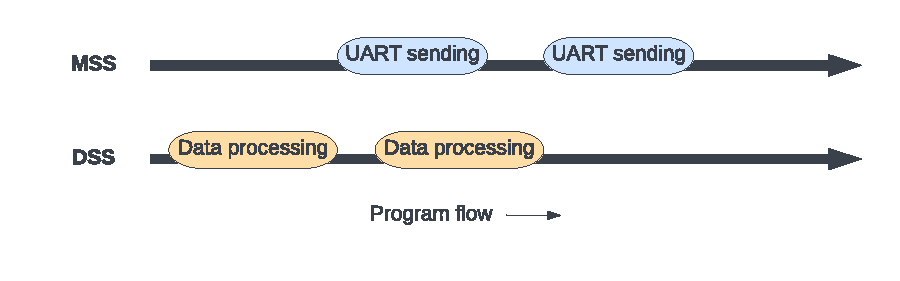
\includegraphics[width=.95\textwidth]{figures/realtime_implementation/timing_diagram.pdf}
\caption{Visual representation of how the two processors are working together to be as efficient as possible.}
\label{fig:uart_timing}
\end{figure}

\begin{figure}[t]
\centering
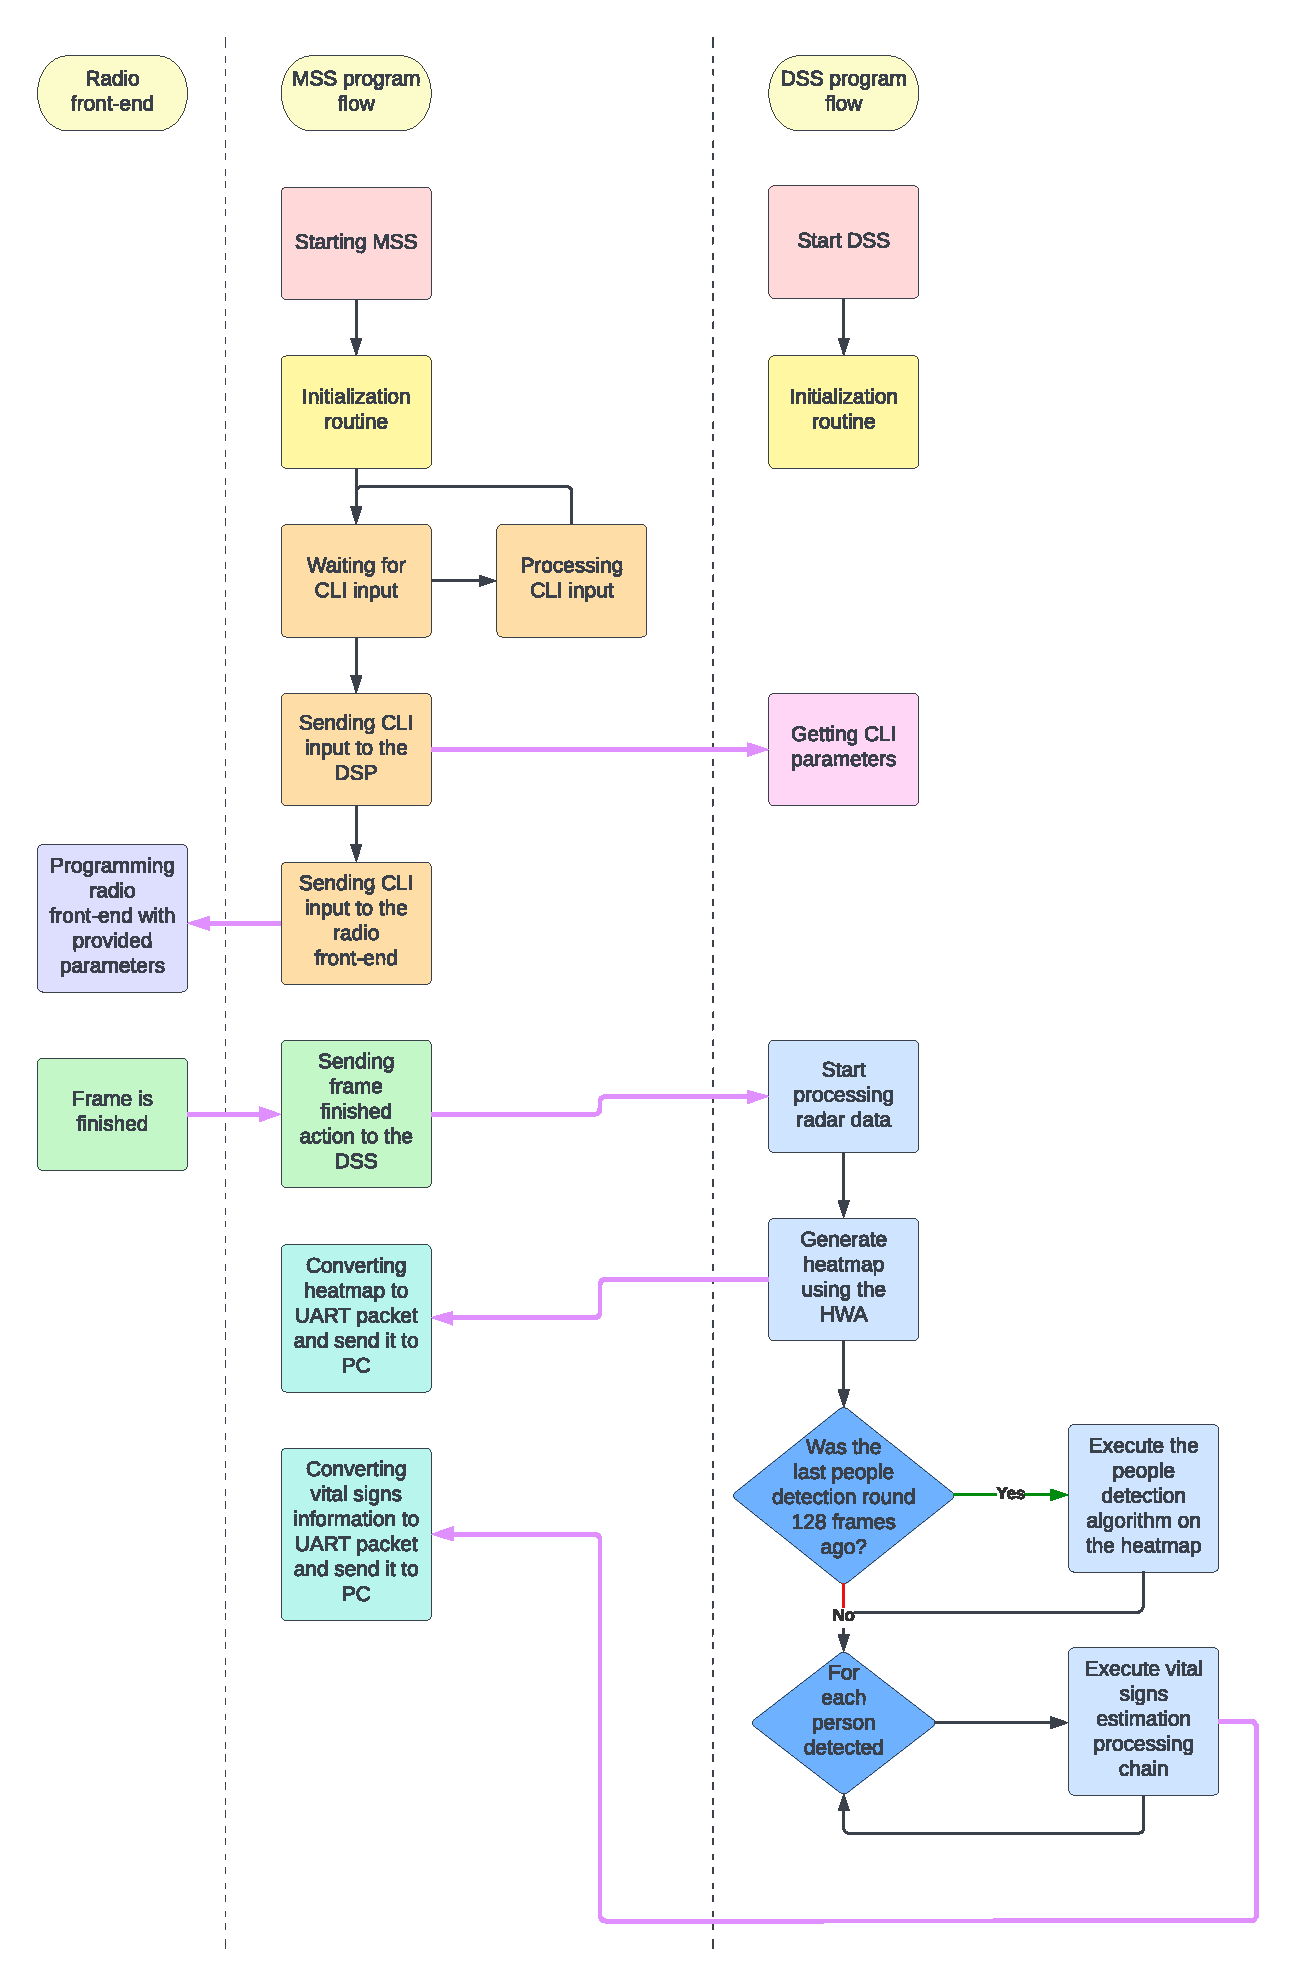
\includegraphics[width=.95\textwidth]{figures/realtime_implementation/Program flow.pdf}
\caption{The program flow from the project in high-level overview. Steps with the same color belong to each other.}
\label{fig:program_flow}
\end{figure}
% Explain:
% - The generic processor
% - The DSP
% - The two processors working together
% - The several hardware accelerators
% - The high-level program flow inside the chip

% Validation of the presented work chapter
\chapter{Validation}
\label{chp:validation}
% Probably the biggest chapter:
% - explain the metrics
% - explain the scenarios
% - display the good and bad results (highlight both)
% - display the high level results

Chapter in which the validation will reside.

% Create conclusions
\chapter{Conclusions}
\label{chp:conclusions}

The aim of this research was to measure multiple peoples heart rate and respiratory rate in real time with FMCW mmWave radar. First, the different existing methods are evaluated. Existing implementations make use of post-processing algorithms to evaluate the data. The existing real-time implementation of this task can only measure one person, because it only makes use of a 1D-FFT. 

The implementation of this thesis is focusing on using the output from the range-azimuth FFT. This output can be further processed to form a 2 dimensional heatmap. Using the data from this heatmap, up to four persons can be detected dynamically. Because all of the complex data stays intact when forming the heatmap, the data needed for the vital signs estimation, the phases of the radar data, can be extracted from the heatmap data for each person detected. For each radar measurements these phases are collected to form a waveform. Two filters can be applied to this waveform, one to extract the heartrate and one to extract the respiration rate. Peak counting is applied to these two waveforms to finally end up with two numbers for each person in the radar frame: a heartrate and a respiration rate.

An important part of this thesis is the validation part. Because a new connection is used to extract the vital signs waveform from the radar data, this method needs to be properly tested. Tests have been done on individual test subjects, but also on two persons at the same time and four persons at the same time. There is also investigated if age, gender or the BMI of a person are connected to the accuracy of the measurement. The accuracy of the heartrate estimation using the sensor compared to the control measurement is around 10\%. The accuracy of the respiratory rate estimation compared to the control measurement is around 8\%. These accuracy's are not as high as we had hoped, but the main focus of this thesis is to show the vital signs of multiple persons can be estimated in real-time using only the embedded hardware. This goal has been reached, all of the calculations mandatory for the vital signs estimation of multiple persons are done on the chip itself. The relation between age, gender or BMI and the accuracy of the sensor cannot be proven using the validation data gathered during this thesis. This could denote that the vital signs estimation using the mmWave method can be used on a broad range of people. 

In Section~\ref{sec:objectives}, the objectives for this project were given in eight points. Almost all of these objectives have been reached, there are only a few which are just partly completed. The chip is able to generate a heatmap from the radar data and detect persons in the heatmap. For these persons, the vital signs are estimated in real-time. The resulting data gets send to the computer, where the data is visualized and saved for later analysis. When doing the validation of this project, the vital sign measurements were compared to medical grade device measurements, to assess the accuracy of the sensor. The tracking of multiple persons is only partly succeeded. When the test subjects are sitting statically, the sensor is able to adjust for small movements. However, if the test subjects are moving a lot, the heatmap becomes so noisy that person tracking is not possible anymore. For the validation part of this project, 16 test subjects have been tested, some even multiple times. This number of subjects gives a good impression of the overall performance of this implementation. One improvement could be the age distribution of the test subjects. No children have been tested for this project, these measurements could have given an interesting view on the performance on smaller chest surfaces.

\section{Future work}
The main improvement on the work done on this thesis are the vital signs estimation algorithms. Because the focus for this project was on the embedded programming and the real-time implementation, the implementation of the vital signs estimation algorithms could not really be improved upon because I lacked the required knowledge. The lower accuracy could be improved by tweaking the parameters of the algorithms, or implementing additional signal processing techniques. 

The code for this project has been written as efficiently as possible. But due to the large code base, and the limited documentation of all the APIs included in the chip, it was very hard to have a grasp on the whole program flow. Developers with more experience on this chip could make the algorithm execution more efficient, by making more use of the specialized hardware in the chip, and the cooperation of the two separate processors. In this project, the DSP is used for all of the calculations, and the ARM processor is used for handling the UART data flow. To make better use of the processing power of the chip, the ARM processor could take over some tasks from the DSP. My estimate is that this could speed up the program by approximately 20\%.

The reach of the sensor could also be improved. For now, the sensor can detect persons up to 2.5 meters away in front of the sensor. To measure for example the heart- and respiration rate of all persons in one room, the range of the sensor must be improved while keeping the accuracy required to estimate the vital signs. This of course also depends on the external requirement that this project is used for.

% Create future work
\include{chapters/futurework}

% Create bibliography
\bibliographystyle{plain} % Please do not change the style of bibliography (yes, it should be `plain`)
\bibliography{bib/references}

% Create appendix
\appendix
\chapter{Tx beamforming}
\label{app:appendix}

Appendix body.

\end{document}
